\documentclass[12pt]{article}
\frenchspacing
\usepackage[utf8x]{inputenc}
\usepackage[T2A]{fontenc}
\usepackage{amsmath}
\usepackage{amsfonts}
\usepackage{amssymb}
\usepackage[russian]{babel}
\usepackage{graphicx}
\usepackage{hyperref}
\usepackage{multirow}
\usepackage[left=2cm,right=2cm,top=2cm,bottom=2cm,bindingoffset=0cm]{geometry}
\author{Рашковецкий М.М., группа 526т}
\date{\today}
\title{Лабораторная работа 2.2.3\\Определение теплопроводности газов при атмосферном давлении}

\newcommand{\degC}{^\circ \text{C}}
\newcommand{\fref}[1]{рис. \ref{#1}}

\begin{document}
	\maketitle
	
	{\parindent=1cm \hangindent=1cm \parskip=0.5cm
	{\bfseries Цель работы:} определение коэффициента теплопроводности воздуха или углекислого газа при атмосферном давлении и разных температурах по теплоотдаче нагреваемой током нити в цилиндрическом сосуде.
	
	\hangindent=1cm
	{\bfseries Оборудование и материалы:} прибор для определения теплопроводности газов; форвакуумный насос; газгольдер с углекислым газом; манометр; магазин сопротивлений; эталонное сопротивление 10 Ом; цифровой вольтметр В7-38; источник питания.\par}
	\section*{Краткая теория}
	
	\indent В задаче о теплопередаче между двумя коаксиальными цилиндрами тепловая мощность, протекающая наружу через цилиндрическую поверхность радиуса $r$ с той же осью записывается как
	\begin{equation}
		\label{eq:heat_stream}
		Q=2\pi r L \varkappa \frac{dT}{dr}.
	\end{equation}
	
	Принимая зависимость коэффициента теплопроводности от температуры степенной
	\begin{equation}
		\label{eq:k_heat_pow}
		\varkappa=\varkappa_2 \left( \frac{T}{T_2} \right) ^\beta,
	\end{equation}
	получаем следующее соотношение:
	\begin{equation}
		\label{eq:k_heat_diff}
		Q \frac{dr}{r} = 2\pi L \frac{\varkappa_2}{T_2^\beta} T^\beta dT.
	\end{equation}
	
	Проинтегрировав его, получим
	\begin{equation}
		\label{eq:k_heat_int}
		Q \ln \frac{r_2}{r_1} = 2\pi L \varkappa_2 \frac{T_2^{\beta+1}-T_1^{\beta+1}}{(\beta+1) T_2^\beta},
	\end{equation}
	откуда
	\begin{equation}
		\label{eq:k_heat_final_accurate}
		\varkappa_2 = \frac{Q}{2\pi L} \frac{(\beta+1) T_2^\beta}{T_2^{\beta+1}-T_1^{\beta+1}} \ln \frac{r_2}{r_1}.
	\end{equation}
	
	В приближении $\Delta T \ll T$ получаем уже разрешимое соотношение:
	\begin{equation}
		\label{eq:k_heat_final}
		\varkappa = \frac{Q}{2\pi L \left( T_2-T_1 \right)} \ln \frac{r_2}{r_1}.
	\end{equation}
	Тут $r_1$, $T_1$ --- радиус и температура нити, $r_2$, $T_2$ --- цилиндра, $L$ --- длина нити и цилиндра.
	
	В работе отношение заменяется на производную, которая расписывается как произведение производных, находимых из результатов измерений:
	\begin{equation}
		\label{eq:k_heat_work}
		\varkappa = \frac{dQ}{dR} \frac{dR}{dT} \frac{1}{2\pi} \ln \frac{r_2}{r_1},
	\end{equation}
	где $R$ --- сопротивление нити.
	
	\section*{Установка}
	
	\begin{figure}[h!]
	\caption{Схема установки}
	\label{fig:scheme}
	\begin{center}
	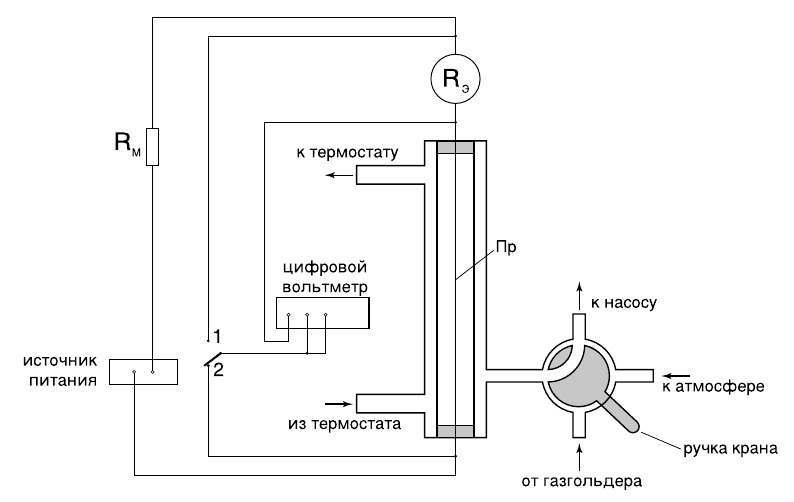
\includegraphics[scale=.6]{scheme.png}
	\end{center}
	\end{figure}
	
	В эксперименте температура нити определяется по изменению электрического сопротивления, температура цилиндра совпадает с температурой термостата, измеряемой его внутренним термометром. Напряжение на проволоке измеряется непосредственно вольтметром в положении 2, ток через неё~--- через напряжение на эталонном сопротивлении в положении 1.
	
	\section*{Ход работы}
	
	\begin{enumerate}
		\item Записали параметры установки: $L=367$ мм, $2r_1=0{,}050$ мм, $2r_2=10$ мм, $R_\text{э}=10$ Ом, материал проволоки --- железо-никелиевый сплав.
		\item Установили на термостате температуру $t=30\degC$ и дождались её установления. \label{hod_loop_begin}
		\item Установили ключ в положение 1, выставили нужное напряжение $U_\text{э}$, подождали, пока оно установится.
		\item Установив ключ в положение 2, измерили соответствующее $U_\text{н}$.
		\item Повторили измерения для разных токов. \label{hod_loop_end}
		\item Повторили пп. \ref{hod_loop_begin}--\ref{hod_loop_end} для других температур.
	\end{enumerate}
	
	\section*{Обработка результатов}
	
	Результаты измерений приведены в таблице \ref{tb:meas_res}. Погрешностью температуры мы пренебрегли, погрешность напряжения приняли $\sigma_U=0{,}001$ В.
	
	\begin{table}[!h]
		\caption{Результаты измерений}
		\label{tb:meas_res}
		\begin{center}
		\begin{tabular}{|c|cccc|}
			\hline
			$t$, $\degC$ & 30 & 40 & 50 & 60 \\
			\hline
			$U_\text{э}$, В & \multicolumn{4}{c|}{$U_\text{н}$, В} \\
			\hline
			0,05 & 0,76 & 0,767 & 0,774 & 0,781 \\
			0,075 & 1,139 & 1,15 & 1,161 & 1,171 \\
			0,1 & 1,52 & 1,534 & 1,548 & 1,563 \\
			0,125 & 1,902 & 1,919 & 1,936 & 1,953 \\
			0,15 & 2,29 & 2,312 & 2,333 & 2,352 \\
			0,175 & 2,675 & 2,7 & 2,724 & 2,746 \\
			0,2 & 3,06 & 3,087 & 3,115 & 3,145 \\
			0,225 & 3,447 & 3,476 & 3,508 & 3,538 \\
			0,25 & 3,833 & 3,868 & 3,897 & 3,933 \\
			\hline
		\end{tabular}
		\end{center}
	\end{table}
	
	Затем я посчитал для каждого $U_\text{н}$ $Q=\frac{U_\text{н} U_\text{э}}{R_\text{э}}$ и $R_\text{н}=R_\text{э} \frac{U_\text{н}}{U_\text{э}}$, посчитал их погрешности и построил графики $Q(R)$ (\fref{fig:graph_QR}).
	
	\begin{figure}[!h]
		\caption{Графики $Q(R)$ для разных температур}
		\label{fig:graph_QR}
		\begin{minipage}{0.5\linewidth}
			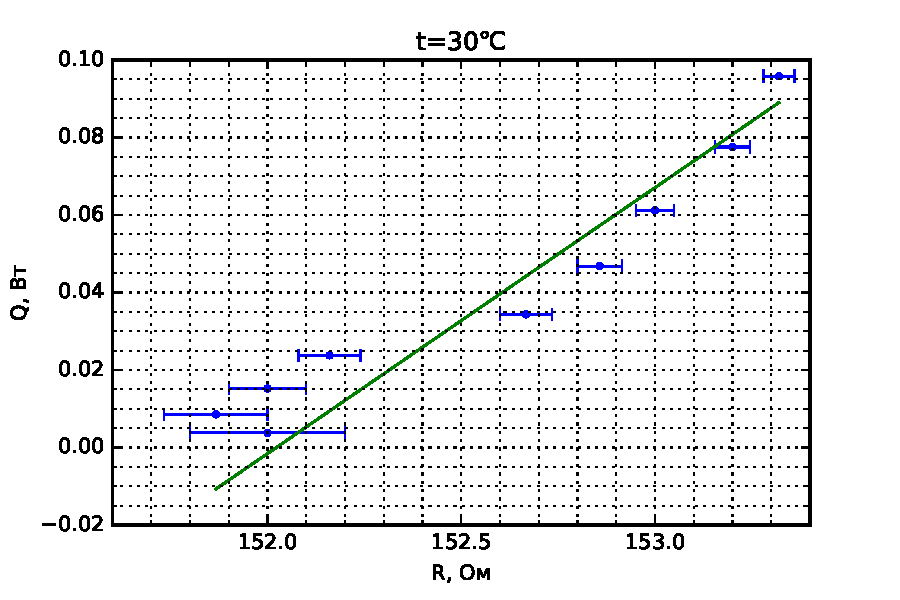
\includegraphics[scale=.6]{graph-QR0.pdf} \\
			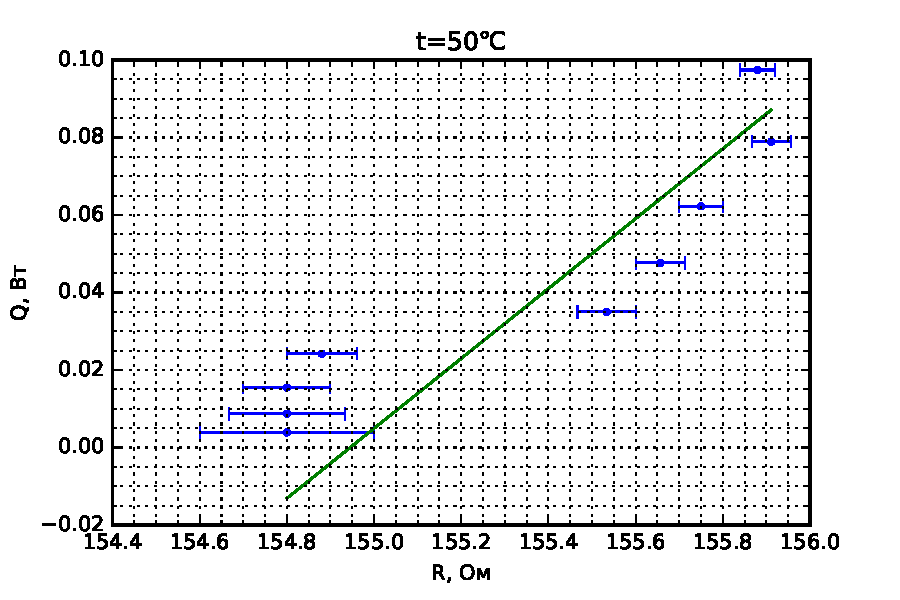
\includegraphics[scale=.6]{graph-QR2.pdf}
		\end{minipage}
		\begin{minipage}{0.5\linewidth}
			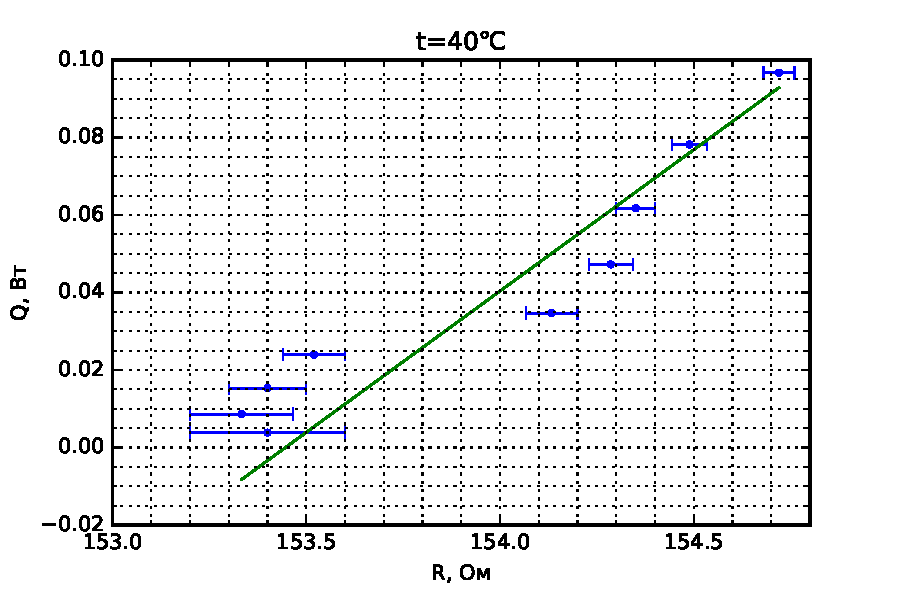
\includegraphics[scale=.6]{graph-QR1.pdf} \\
			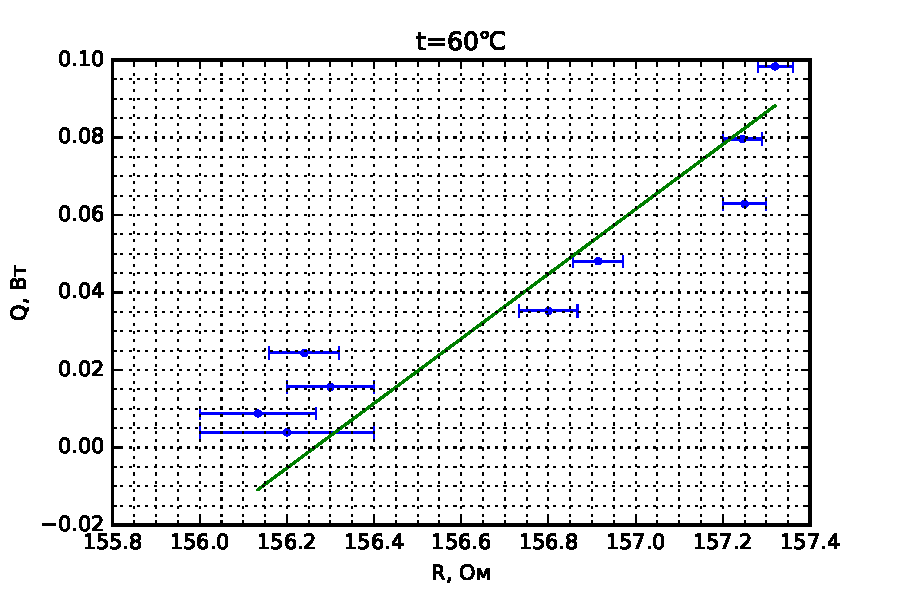
\includegraphics[scale=.6]{graph-QR3.pdf}
		\end{minipage}
	\end{figure}
	
	На графиках также изображена линейная аппроксимация, которая использовалась, чтобы найти $R_0$ --- сопротивление при $Q=0$, т.е. при температуре термостата, и $\frac{dQ}{dR}$ в той же точке. Параметры аппроксимаций приведены в таблице \ref{tb:approx_params}.
	
	\begin{table}[!h]
		\caption{Параметры аппроксимации}
		\label{tb:approx_params}
		\begin{center}
		\begin{tabular}{|c|cccc|}
			\hline
			$t$, $\degC$ & 30 & 40 & 50 & 60 \\
			\hline
			$R_0$, Ом & 152,02$\pm$0,12 & 153,45$\pm$0,13 & 154,95$\pm$0,17 & 156,26$\pm$0,15 \\
			$\frac{dQ}{dR}$, $\frac{\text{Вт}}{\text{Ом}}$ & 0,069$\pm$0,008 & 0.073$\pm$0,010 & 0,09$\pm$0,02 & 0,084$\pm$0,015 \\
			\hline
		\end{tabular}
		\end{center}
	\end{table}
	
	По этим данным я построил график $R_0(t)$ (\fref{fig:graph_Rt}).
	
	\begin{figure}[!h]
		\caption{График $R_0(t)$}
		\label{fig:graph_Rt}
		\begin{center}
		 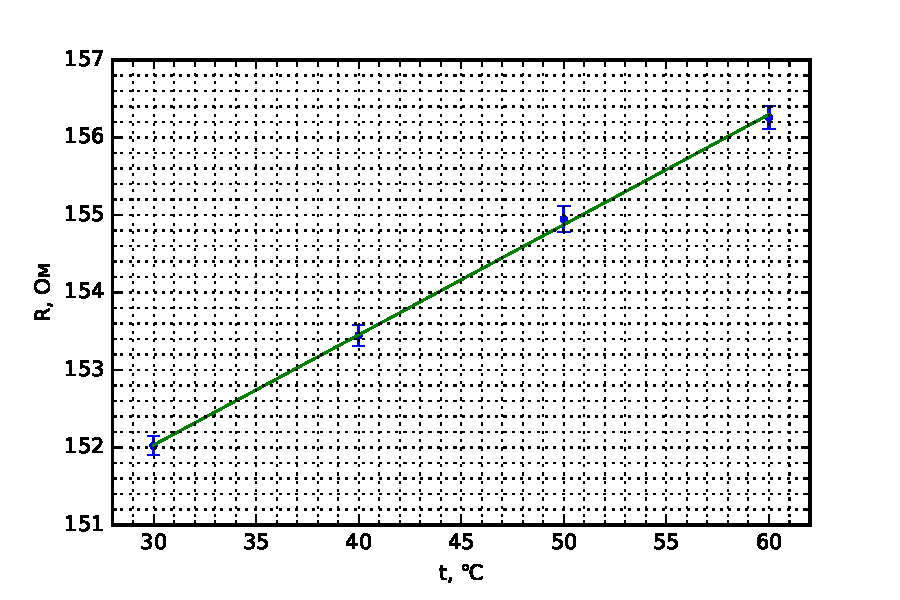
\includegraphics[scale=.8]{graph-Rt.pdf}
		\end{center}
	\end{figure}
	
	Он был также аппроксимирован линейно, параметры: $R_{0\degC}=(147{,}8\pm 0{,}3)$ Ом, $\frac{dR}{dT}=(0{,}142\pm 0{,}006) \frac{\text{Ом}}{\text{K}}$, соответственно температурный коэффициент сопротивления получился $\alpha=(9{,}6\pm 0{,}4) \cdot 10^{-4} \,\text{K}^{-1}$, что по порядку величины совпадает с табличными данными для металлов.
	
	Затем по \eqref{eq:k_heat_work} был посчитан коэффициент теплопроводности. Результаты приведены в таблице \ref{tb:res_kappa} и на \fref{fig:graph_KT}.
	
	\begin{table}[!h]
		\caption{Коэффициент теплопроводности}
		\label{tb:res_kappa}
		\begin{center}
		\begin{tabular}{|c|cccc|}
			\hline
			$t$, $\degC$ & 30 & 40 & 50 & 60 \\
			\hline
			$\varkappa, \frac{\text{Вт}\cdot \text{К}}{\text{м}^2}$ & 0,022$\pm$0,003 & 0,024$\pm$0,003 & 0,030$\pm$0,006 & 0,027$\pm$0,005 \\
			\hline
		\end{tabular}
		\end{center}
	\end{table}
	
	\begin{figure}[!h]
		\caption{График $\ln \varkappa(\ln T)$}
		\label{fig:graph_KT}
		\begin{center}
		 \includegraphics[scale=.8]{graph-KT.pdf}
		\end{center}
	\end{figure}
	
	По порядку величины результаты совпадают с табличными, однако разброс соответствующих температур больше, чем должен быть (где-то от $-20 \degC$ до $100 \degC$).
	
	Из графика я получил значение для степени зависимости $\beta$:
	\begin{equation}
		\label{eq:beta}
		\beta=2{,}5\pm2{,}2 
	\end{equation}
	
	Точность результата фактически не позволяет ничего сказать. Возможные причины такого плохого результата: мы не дождались установления теплового равновесия, утечки тепла через саму проволоку, разница температур была слишком большой для приближённой формулы \eqref{eq:k_heat_final} и следовало использовать \eqref{eq:k_heat_final_accurate}, хотя это было бы сложно.
	
\end{document}
